This section provides details on the implementation of various Unit Hydrographs. An overview of the 8 UHs is given in Table \ref{tab:sm3_1}. Computational implementation of each UH is given in sections \ref{sec:sm3_1} to \ref{sec:sm3_8}. Unit Hydrograph files can be found in ''./MARRMoT/Models/Unit Hydrograph files/''.

% Table generated by Excel2LaTeX from sheet 'Sheet1'
\begin{table}[ht!]
  \centering
  \caption{Overview of Unit Hydrograph schemes implemented in MARRMoT}
\hspace*{-5em}    
\begin{tabular}{rp{10.57em}lrl}
    \toprule
    \multicolumn{1}{p{6.215em}}{\textbf{File name}} & \textbf{Inputs} & \multicolumn{1}{p{8.645em}}{\textbf{Diagram}} & \multicolumn{1}{p{8.43em}}{\textbf{Description }} & \multicolumn{1}{p{6.07em}}{\textbf{In model ...}} \\
    \midrule
    \multicolumn{1}{p{6.215em}}{uh\_1\_half} & 1: amount to be routed & \multirow{3}[1]{*}{ \begin{minipage}{3cm} 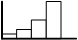
\includegraphics[height=1.3cm]{./SM3/uh1} \end{minipage}} & \multicolumn{1}{l}{Exponentially} & 7 \\
          & 2: time base &       & \multicolumn{1}{l}{increasing} &  \\
          & 3: $\Delta$t &       & \multicolumn{1}{l}{scheme} &  \\
          & \multicolumn{1}{l}{} &       &       &  \\
    \multicolumn{1}{p{6.215em}}{uh\_2\_full} & 1: amount to be routed & \multirow{3}[0]{*}{ \begin{minipage}{3cm} 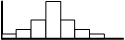
\includegraphics[height=1.3cm]{./SM3/uh2} \end{minipage} } & \multicolumn{1}{p{8.43em}}{Exponential} & 7 \\
          & 2: time base (doubled inside the function) &       & \multicolumn{1}{p{8.43em}}{triangular scheme} &  \\
          & 3: $\Delta$t &       &       &  \\
          & \multicolumn{1}{l}{} &       &       &  \\
    \multicolumn{1}{p{6.215em}}{uh\_3\_half} & 1: amount to be routed & \multirow{3}[0]{*}{ \begin{minipage}{3cm} 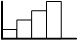
\includegraphics[height=1.3cm]{./SM3/uh3} \end{minipage} } & \multicolumn{1}{p{8.43em}}{Triangular scheme:} & \multicolumn{1}{p{6.07em}}{13, 15, 21, 26} \\
          & 2: time base &       & \multicolumn{1}{p{8.43em}}{linearly increasing} & 34 \\
          & 3: $\Delta$t &       &       &  \\
          & \multicolumn{1}{l}{} &       &       &  \\
    \multicolumn{1}{p{6.215em}}{uh\_4\_full} & 1: amount to be routed & \multirow{3}[0]{*}{ \begin{minipage}{3cm} 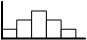
\includegraphics[height=1.3cm]{./SM3/uh4} \end{minipage} } & \multicolumn{1}{p{8.43em}}{Triangular scheme:} & \multicolumn{1}{p{6.07em}}{0 (template), } \\
          & 2: time base &       & \multicolumn{1}{p{8.43em}}{linearly increasing} & \multicolumn{1}{p{6.07em}}{16, 37, } \\
          & 3: $\Delta$t &       & \multicolumn{1}{p{8.43em}}{and decreasing} & \multicolumn{1}{p{6.07em}}{nn (example)} \\
          & \multicolumn{1}{l}{} &       &       &  \\
    \multicolumn{1}{p{6.215em}}{uh\_5\_half} & 1: amount to be routed & \multirow{3}[0]{*}{ \begin{minipage}{3cm} 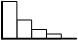
\includegraphics[height=1.3cm]{./SM3/uh5} \end{minipage} } & \multicolumn{1}{p{8.43em}}{Exponentially} & 5 \\
          & 2: time base &       & \multicolumn{1}{p{8.43em}}{decreasing} &  \\
          & 3: $\Delta$t &       & \multicolumn{1}{p{8.43em}}{scheme} &  \\
          & \multicolumn{1}{l}{} &       &       &  \\
    \multicolumn{1}{p{6.215em}}{uh\_6\_gamma} & 1: amount to be routed & \multirow{4}[0]{*}{ \begin{minipage}{3cm} 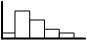
\includegraphics[height=1.3cm]{./SM3/uh6} \end{minipage} } & \multicolumn{1}{p{8.43em}}{Gamma function-} & 40 \\
          & 2: gamma parameter [-] &       & \multicolumn{1}{p{8.43em}}{based} &  \\
          & 3: time for flow to reduce by factor e [d] &       &       &  \\
          & 4: length of time series &       &       &  \\
          & \multicolumn{1}{l}{} &       &       &  \\
    \multicolumn{1}{p{6.215em}}{uh\_7\_uniform} & 1: amount to be routed & \multirow{3}[1]{*}{ \begin{minipage}{3cm} 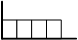
\includegraphics[height=1.3cm]{./SM3/uh7} \end{minipage} } & \multicolumn{1}{p{8.43em}}{Uniform} & 39 \\
          & 2: time base &       & \multicolumn{1}{p{8.43em}}{distribution} &  \\
          & 3: $\Delta$t  &       &       &  \\
          & \multicolumn{1}{l}{} &       &       &  \\

\multicolumn{1}{p{6.215em}}{uh\_8\_delay} & 1: amount to be delayed & \multirow{3}[1]{*}{ \begin{minipage}{3cm} 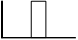
\includegraphics[height=1.3cm]{./SM3/uh8} \end{minipage} } & \multicolumn{1}{p{8.43em}}{Pure time} & 5 \\
          & 2: time delay &       & \multicolumn{1}{p{8.43em}}{delay} &  \\
          & 3: $\Delta$t  &       &       &  \\

    \bottomrule
    \end{tabular}%
  \label{tab:sm3_1}%
\end{table}%

%UH1
\newpage
\subsection{Code: uh\_1\_half} \label{sec:sm3_1}
This section provides the computational implementation of a unit hydrograph with an increasing exponential distribution of flows. \\

\begin{tabular}{ll}
	File location & 	./MARRMoT/Models/Unit Hydrograph files/uh\_1\_half \\
	References & 	E.g. GR4J \citep{Perrin2003} \\
\end{tabular}

\bigskip
\lstinputlisting[style=Matlab-editor]{"C:/Users/wk14463/Google Drive/PhD/Calculations/10. MARRMoT - review/Models/Unit hydrograph files/uh_1_half.m"}

%UH2
\subsection{Code: uh\_2\_full} \label{sec:sm3_2}
This section provides the computational implementation of a unit hydrograph with an exponential triangular distribution of flows. \\

\begin{tabular}{ll}
	File location & 	./MARRMoT/Models/Unit Hydrograph files/uh\_2\_full \\
	References & 	E.g. GR4J \citep{Perrin2003} \\
\end{tabular}

\bigskip
\lstinputlisting[style=Matlab-editor]{"C:/Users/wk14463/Google Drive/PhD/Calculations/10. MARRMoT - review/Models/Unit hydrograph files/uh_2_full.m"}

%UH3
\subsection{Code: uh\_3\_half} \label{sec:sm3_3}
This section provides the computational implementation of a unit hydrograph with an linearly increasing distribution of flows. \\

\begin{tabular}{ll}
	File location & 	./MARRMoT/Models/Unit Hydrograph files/uh\_3\_half \\
	References & 	E.g. FLEX-Topo \citep{Savenije2010}
\end{tabular}

\bigskip
\lstinputlisting[style=Matlab-editor]{"C:/Users/wk14463/Google Drive/PhD/Calculations/10. MARRMoT - review/Models/Unit hydrograph files/uh_3_half.m"}

%UH4
\subsection{Code: uh\_4\_full} \label{sec:sm3_4}
This section provides the computational implementation of a unit hydrograph with an linear triangular distribution of flows. \\

\begin{tabular}{ll}
	File location & 	./MARRMoT/Models/Unit Hydrograph files/uh\_4\_full \\
	References & 	E.g. HBV-96 \citep{Lindstrom1997} \\
\end{tabular}

\bigskip
\lstinputlisting[style=Matlab-editor]{"C:/Users/wk14463/Google Drive/PhD/Calculations/10. MARRMoT - review/Models/Unit hydrograph files/uh_4_full.m"}

%UH5
\subsection{Code: uh\_5\_half} \label{sec:sm3_5}
This section provides the computational implementation of a unit hydrograph with an decreasing exponential distribution of flows. \\

\begin{tabular}{ll}
	File location & 	./MARRMoT/Models/Unit Hydrograph files/uh\_5\_half \\
	References & 	E.g. IHACRES \citep{Littlewood1997,Croke2004} \\
\end{tabular}

\bigskip
\lstinputlisting[style=Matlab-editor]{"C:/Users/wk14463/Google Drive/PhD/Calculations/10. MARRMoT - review/Models/Unit hydrograph files/uh_1_half.m"}

%UH6
\subsection{Code: uh\_6\_gamma} \label{sec:sm3_6}
This section provides the computational implementation of a unit hydrograph with a gamma distribution of flows. \\

\begin{tabular}{ll}
	File location & 	./MARRMoT/Models/Unit Hydrograph files/uh\_6\_gamma \\
	References & 	E.g. SMAR \citep{OConnell1970,Tan1996} \\
\end{tabular}

\bigskip
\lstinputlisting[style=Matlab-editor]{"C:/Users/wk14463/Google Drive/PhD/Calculations/10. MARRMoT - review/Models/Unit hydrograph files/uh_6_gamma.m"}

%UH7
\subsection{Code: uh\_7\_uniform} \label{sec:sm3_7}
This section provides the computational implementation of a unit hydrograph with a uniform distribution of flows. \\

\begin{tabular}{ll}
	File location & 	./MARRMoT/Models/Unit Hydrograph files/uh\_7\_uniform \\
	References & 	E.g. MCRM \citep{Moore2001a,Moore2001} \\
\end{tabular}

\bigskip
\lstinputlisting[style=Matlab-editor]{"C:/Users/wk14463/Google Drive/PhD/Calculations/10. MARRMoT - review/Models/Unit hydrograph files/uh_7_uniform.m"}

%UH8
\subsection{Code: uh\_8\_delay} \label{sec:sm3_8}
This section provides the computational implementation of a unit hydrograph that delays flow without transforming it. \\

\begin{tabular}{ll}
	File location & 	./MARRMoT/Models/Unit Hydrograph files/uh\_8\_delay \\
	References & 	E.g. IHACRES \citep{Littlewood1997,Croke2004} \\
\end{tabular}

\bigskip
\lstinputlisting[style=Matlab-editor]{"C:/Users/wk14463/Google Drive/PhD/Calculations/10. MARRMoT - review/Models/Unit hydrograph files/uh_8_delay.m"}

